\newpage
\changeindent{0cm}
\section{要素技術}
\changeindent{2cm}


%%%%%%%%%%%%%%%%%%%%%%%%%%%%%%
% 3.1. BERT
% https://arxiv.org/abs/1810.04805
% 3.2 SARC データセット
%%%%%%%%%%%%%%%%%%%%%%%%%%%%%%
本章では,本研究で使用した要素技術とデータセットについて記述する.
\subsection{BERT}

Bidirectional Encoder Representations from Transformers (BERT) \cite{devlin-etal-2019-bert} は,2018 年 10 月に Jacob Devlin らが発表した Transformer \cite{NIPS2017_3f5ee243} による双方向のエンコーダーを用いた言語モデルである.
公開当時に様々な自然言語処理タスクで state-of-the-art の性能を示した.
文章を文頭と文末の双方向から学習することによって文脈の理解を可能としている.
\par 
BERT は大規模コーパスを用いて事前学習することでモデルの性能を向上させている.
事前学習には,[MASK] トークンに当てはまる単語を予測する Masked Language Modeling と,入力された 2 文が意味的に連続するかを予測する Next Sentence Prediction の 2 つのタスクが用いられる.
\par
BERT は様々な事前学習済みモデルが発表されており,ファインチューニングすることで各タスクに応用可能である.
図 \ref{fig:31_bert_model} はその概略図を表している.
本研究では,英語の事前学習済みモデルである bert-base-uncased \footnote{\url{https://huggingface.co/bert-base-uncased}} を使用した.
このモデルは本のデータセットである BookCorpus \cite{bookcorpus} と Wikipedia \footnote{\url{https://en.wikipedia.org/wiki/Main_Page}} の英語記事を用いて事前学習している.
BookCorpus は約 8 億語,Wikipedia は約 2 億 5 千万語を含んでいる.
またこのモデルは英語の大文字と小文字の区別をしない.
モデルの層数は 12 層,隠れ層の次元数は 768 次元,最大入力長は 512 トークンである.


%%% figure BERT のファインチューニング
\begin{figure}[b]
 	\begin{center}
		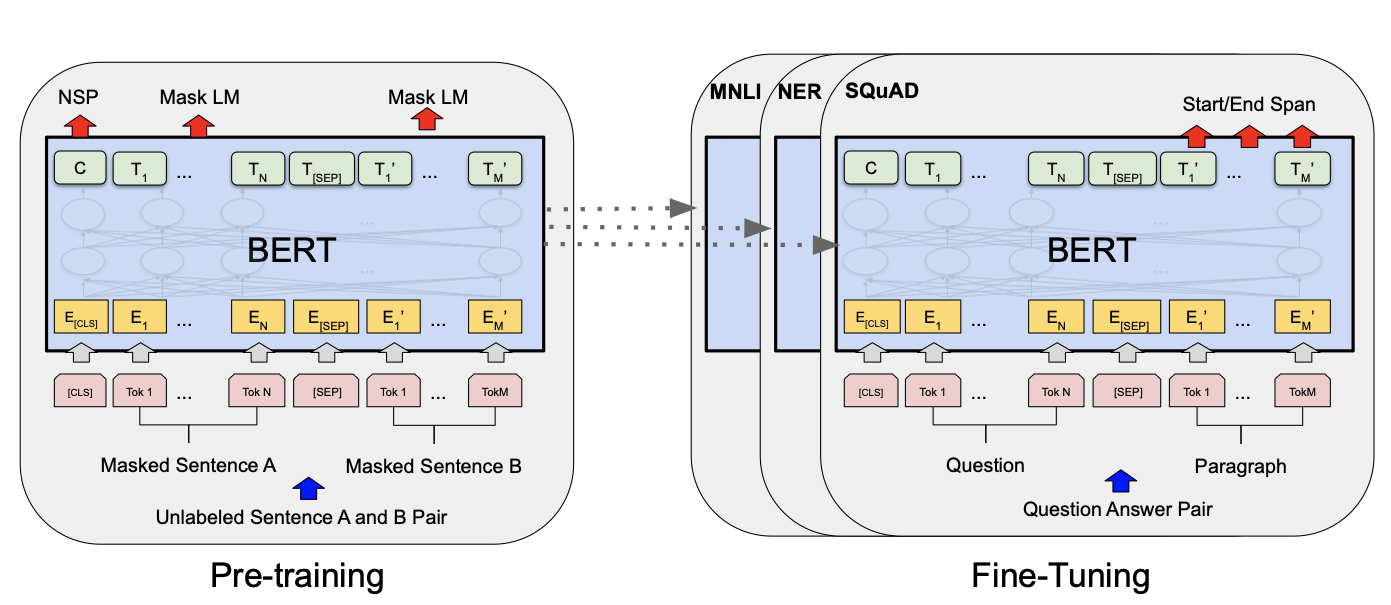
\includegraphics[width=\linewidth]{./figure/31_BERT_figure1.png}
		\caption{BERT のファインチューニングの概要図(文献 \cite{devlin-etal-2019-bert} Figure 1 より引用)}
		\label{fig:31_bert_model}
	\end{center}
\end{figure}
% end figure

BERT に文を入力する際は,まず tokenizer を用いて文をトークンに分割し,ID に変換する.
本研究では BERT モデルと同じ bert-base-uncased の tokenizer を使用した.
この tokenizer は WordPiece \cite{wu2016googles} モデルを用いて,文を単語よりも細かいサブワードに分割する.
これによって未知語を分解し,削減することができる.
BERT には特殊トークンが用意されており,入力の際は変換した ID 列の先頭に [CLS] トークンを,各文の末尾に該当する位置に [SEP] トークンを挿入する.
入力に対して BERT は各トークンに対応する分散表現を出力する.
このとき [CLS] トークンに対応する分散表現は入力された文全体の特徴を捉えており,分類問題に使用することができる.
